%% Thesis template
%% PMC, University of Minho
%% if required, comment unused packages
\documentclass[12pt,english,oneside]{book}
% \usepackage[portuguese]{babel}
% \usepackage[utf8]{inputenc} 
\usepackage{times}
\usepackage[T1]{fontenc}
\usepackage[latin1]{inputenc}
\usepackage{a4wide}
\usepackage{fancyhdr}
\pagestyle{fancy}
\usepackage{subfigure}
\usepackage{float}
\usepackage{graphicx}
\usepackage{setspace}
\usepackage{cite}\onehalfspacing

\makeatletter

%%%%%%%%%%%%%%%%%%%%%%%%%%%%%% LyX specific LaTeX commands.
%% Bold symbol macro for standard LaTeX users
\newcommand{\boldsymbol}[1]{\mbox{\boldmath $#1$}}

\floatstyle{ruled}
\newfloat{algorithm}{tbp}{loa}
\floatname{algorithm}{Algorithm}

%%%%%%%%%%%%%%%%%%%%%%%%%%%%%% Textclass specific LaTeX commands.
 \usepackage{verbatim}
 \newenvironment{lyxlist}[1]
   {\begin{list}{}
     {\settowidth{\labelwidth}{#1}
      \setlength{\leftmargin}{\labelwidth}
      \addtolength{\leftmargin}{\labelsep}
      \renewcommand{\makelabel}[1]{##1\hfil}}}
   {\end{list}}

%%%%%%%%%%%%%%%%%%%%%%%%%%%%%% User specified LaTeX commands.
\usepackage{color}
\usepackage{colortbl}
\usepackage{url}
\input{epsf}
\newcommand{\single}{\renewcommand\baselinestretch{1.0}}
\newcommand{\onehalf}{\renewcommand\baselinestretch{1.5}}
\newcommand{\double}{\renewcommand\baselinestretch{2.0}}
\fancyhead{}
\fancyhead[LE]{\slshape \leftmark}
\fancyhead[RO]{\slshape \rightmark}
\cfoot{\thepage}
\setlength{\parskip}{2mm}

\usepackage{babel}
\makeatother
\begin{document}
\begin{minipage}[c]{1.0\columnwidth}%
\begin{doublespace}
\vspace{2cm}
\begin{center}{\huge A new Framework to enable rapid innovation in Cloud Datacenter through a SDN approach.}\end{center}{\huge \par}
\end{doublespace}

\vspace{2cm}
\begin{center}{\large Jos\'{e} Teixeira}\end{center}{\large \par}
\vspace{2cm}

\begin{quote}
\begin{center}A thesis submitted to the University of Minho in the
subject of Informatics, for the degree of
% or Doctor of Philosophy 
Master of Science, under scientific supervision of Prof. Stefano Giordano and Prof. Alexandre Santos\end{center}\vspace{3cm}

\end{quote}
\begin{singlespace}
\begin{center}University of Minho\end{center}

\begin{center}School of Engineering\end{center}

\begin{center}Department of Informatics\end{center}
\end{singlespace}

\begin{center}{\large September, 2013}\end{center}\end{minipage}%
\thispagestyle{empty}

\pagenumbering{roman}


\newpage


\chapter*{Acknowledgments}

\addcontentsline{toc}{chapter}{Acknowledgments}

\noindent I would like...

\medskip{}
\noindent I also...

\chapter*{Abstract}

\addcontentsline{toc}{chapter}{Abstract}

\begin{singlespace}
\hspace{0.6cm}
In the last years, the widespread of Cloud computing as the main paradigm to deliver a large plethora of virtualized services significantly increased the complexity of Datacenters management and raised new performance issues for the intra-Datacenter network.
Providing heterogeneous services and satisfying users' experience is really challenging for Cloud service providers, since system (IT resources) and network administration functions are definitely separated.

As the Software Defined Networking (SDN) approach seems to be a promising way to address innovation in Datacenters, the thesis presents a new framework that allows to develop and test new OpenFlow--based controllers for Cloud Datacenters.
More specifically, the framework enhances both Mininet (a well--known SDN emulator) and POX (a Openflow controller written in python), with all the extensions necessary to experiment novel control and management strategies of IT and network resources.

... talk about obtained results and conclusions(not finished yet, complete when you finish everything)

\end{singlespace}

\paragraph{Keywords:}
Datacenter, Cloud, SDN, OpenFlow.

\newpage

\addcontentsline{toc}{chapter}{Contents}\tableofcontents{}

\clearpage

\chapter*{List of Acronyms}

\addcontentsline{toc}{chapter}{List of Acronyms}

\markboth{LIST OF ACRONYMS}{LIST OF ACRONYMS}

\begin{lyxlist}{00.00.0000}
\begin{singlespace}
\item [DC]Datacenter
\item [IP]Internet Protocol 
\item [IT]Information Technology
\item [OF]Openflow
\item [QoS] Quality of Service
\item [SDN]Software Defined Networking
\item [VM]Virtual Machine
\item Add as needed...
\end{singlespace}
\end{lyxlist}


\addcontentsline{toc}{chapter}{List of Figures}\listoffigures


\addcontentsline{toc}{chapter}{List of Tables}\listoftables


\setcounter{page}{0}

\pagenumbering{arabic}


\chapter{Introduction\label{cha:introduction}}

\section{Introduction}
\hspace{0.6cm}

A Cloud DC consists of virtualized resources that are dynamically allocated, in a seamless and automatic way, to a plethora of heterogeneous applications.
In Cloud DCs, services are no more tightly bounded to physical servers, as occurred in traditional DCs, but are provided by Virtual Machines that can migrate from a physical server to another increasing both scalability and reliability.
Software virtualization technologies allow a better usage of DC resources; DC management, however, becomes much more difficult, due to the strict separation between systems (\textit{i.e.}, server, VMs and virtual switches) and network (\textit{i.e.}, physical switches) administration.

Moreover, new issues arise, such as isolation and connectivity of VMs.
Services performance may suffer from the fragmentation of resources as well as the rigidity and the constraints imposed by the intra-DC network architecture (usually a multilayer 2-tier or 3-tier fat-tree composed of Edge, Aggregation and Core switches\cite{dc_arch}).
Therefore, Cloud service providers (\textit{e.g.},\cite{amazon}) ask for a next generation of intra-DC networks meeting the following features: 1) efficiency, \textit{i.e.}, high server utilization; 2) agility, \textit{i.e.}, fast network response to server/VMs provisioning; 3) scalability, \textit{i.e.}, consolidation and migration of VMs based on applications' requirements; 4) simplicity, \textit{i.e.}, performing all those tasks easily\cite{baldonado}.

In this scenario, a recent approach to programmable networks (\textit{i.e.}, Software-Defined Networking) seems to be a promising way to satisfy DC network requirements\cite{ibmnec}. 
Unlike the classic approach where network devices forward traffic according to the adjacent devices, SDN is a new network paradigm that decouples routing decisions (control plane) from the traffic forwarding (data plane). This routing decisions are made by a programmable centralized intelligence called controller that helps make this architecture more dynamic, automated and manageable.

Following the SDN--based architecture the most deployed SDN protocol is OpenFlow\cite{openflow}\cite{onf}, and it is the open standard protocol to communicate and control OF-compliant network devices.
Openflow allows a controller to install into OF--compliant network devices forwarding rules which are defined by the administrator/network engineer and match specific traffic flows.

Since SDN allows to re-define and re-configure network functionalities, the basic idea is to introduce an SDN-cloud-DC controller that enables a more efficient, agile, scalable and simple use of both VMs and network resources.
Nevertheless, before deploying the novel architectural solutions, huge test campaigns must be performed in experimental environments reproducing a real DC.
To this aim, a novel framework is introduced that allows to develop and assess novel SDN-Cloud-DC controllers, and to compare the performance of control and management strategies jointly considering both IT and network resources\cite{im2013}.

TODO:should describe better openflow and SDN
% \begin{quote}''OpenFlow allows, for the first time, an external control plane to abstract the entire underlying network fabric so that fabric is universally addressable and all topology and state information is commonly managed''{ --- \textup{ Jason Matlof}, vice president of marketing at Big Switch}\end{quote}

% \newpage
\section{Motivation and objectives\label{sec:motobj}}
\hspace{0.6cm}

Although SDN came as a solution to fulfill the network requirements of the DCs, the only point of interaction with the IT resources is the generated traffic.
By definition SDN does not go further, but if there could be a controller that manages both IT and network resources, all the information could be shared easily and both of them could greatly benefit: the network could start to anticipate IT actions and adapt itself to have higher performance, more redundancy, etc; the IT because the resources could be better managed so that the network, not only stops being the bottleneck, but actually helps the IT complete the tasks faster and without affecting adjacent resources.

When developing an Openflow controller, the administrator/network engineer goals are to implement the desired behaviour and to test it (making sure it suits the requirements).
The currently available controllers already provide some abstraction, which varies according to the type of programming language, but they are still too low level to allow rapid innovation. 
Following the implementation, tests campaigns must be performed and for it a controlled environment should be set.
Although Openflow allows the use of slices of the real network for testing purposes, it is more convenient to use an emulator since the DC size can be dynamic, different scenarios can be easily produced and it only needs a single computer -- Mininet is such an emulator.
Despite its flexible API, Mininet does not provide any type of traffic generator and is not DC--oriented: poor topology generation regarding DCs; no support for VMs;

A whole framework composed by a modified OF controller that allows the access to both IT and network resources through an easy-to-use but full featured API, and a testing environment that communicates with it to provide a real DC emulation is the the main objective.
With this is is expected to endue the administrator/network engineer with all the tools needed to quickly develop, test and deploy VM and network management strategies into a DC.

% When the admin wants to try new DC VM allocation algorithms, first it takes to long to develop since the current controllers are still low level, and second if they want to test, or they try on their own DC (which could compromise the normal functioning and unless they try on a small part of the DC the result wont be accurate since they would be influences by the usual workload.
% Or they would use simulators(the problem with simulator is that usually you have to rewrite the algorithms that you will implement, and the results might not be accurate (correspond to the real environment)).
% At the same time, a whole framework that provides support to develop and test only the logic that the admin wants would also be cool, since they could focus on making new VM allocations that consider multiple factor (this is where OF helps since it has info about network)
% Maybe also talk a little about allowing to be easily expandable, extended.

% \begin{itemize}
% 	\item Understanding the basic features of SDN paradigm
% 	\item Studying the problematics in cloud DC VM allocations
% 	\item Apply the SDN paradigm to better exploit the DC resources
% 	\item Develop a framework for Cloud Datacenter emulation and new VM allocation policies
% 	\item ...
% \end{itemize}


\section{Thesis layout}
\hspace{0.6cm}

This thesis is structured into five chapters: the present Chapter \ref{cha:introduction} is a brief introduction of the proposed work, its motivation and objectives; the second is the state of art, it addresses the currently available solutions relating innovation in DCs, OF controllers and VM allocation and migration algorithms; the third one fully describes the framework, its evolution, extensions and how it can be used; in the forth chapter is presented the framework validation and performance tests; and in the last chapter are made conclusions about the developed work, as well as suggestions for future work.



\chapter{State of art \label{cha:stateofart} }

\section{Available solutions}

A number of research efforts have focused on novel solutions for emulation/simulation of Cloud DCs.
The available solutions provide a reference and material to analise and explore the concepts addressed along this thesis. 
This section presents and overview of them, highlighting their architecture, features and limitations.

\subsection{CloudSim}
\hspace{0.6cm}

Calheiros et al.\cite{cloudsim} proposed a Java-based platform, called Cloudsim, that allows to estimate cloud servers performance using a workflow model to simulate applications behaviour.
By providing a framework for managing most key aspect of a Cloud infrastructure (DC hardware and software, VM placement algorithm, Applications for VM, Storage access, Bandwidth provisioning) and by taking into consideration factors as energy-aware computational resources and costs, it helps to identify possible bottlenecks and improve overall efficiency.

Regarding the network aspect of Clousim, Garg et al.\cite{cloudsim2} extended such a system with both a new intra--DC network topology generator and a flow--based approach for collecting the value of network latency. However, in such a simulator, networks are considered only to introduce delay, therefore it is not possible to calculate other parameters (\textit{e.g.}, Jitter).
A SDN extension for Cloudsim as already been thought, Kumar et al.\cite{cloudsim3}, but it still just an architecture design, meaning it has not been implemented yet.

Although it allows to predict how the management strategies will behave, as a simulator, it does not allow to run real applications and deploying the tested management logic in a real environment still requires everything to be developed.

\subsection{FPGA Emulation}
\hspace{0.6cm}

Ellithorpe et al.\cite{box} proposed, a FPGA emulation platform that allows to emulate up-to 256 network nodes on a single chip.
\begin{quotation}
''Our basic approach to emulation involves constructing a model of the target architecture by composing simplified hardware models
of key datacenter building blocks, including switches, routers, links, and servers. Since models in our system are implemented in programmable hardware, designers have full control over emulated buffer sizes, line rates, topologies, and many other network properties.''

\hfill Ellithorpe et al.\cite{box}
\end{quotation}

This platform also allows the emulation of full SPARC v8 ISA compatible processor, which along with full system control provides a greater system visibility.
However, hardware programming skills might be a requirement and the cost of a single board is approximately 2, 000 dollars making this solution less attractive than ones based on just open--source software.

\subsection{Meridian}
\hspace{0.6cm}

Following the new shiny SDN paradigm, Banikazemi et al.\cite{meridian} proposed Meridian, an SDN--based controller
framework for cloud services in real environments.

\begin{figure}[htbp]
        \centering
        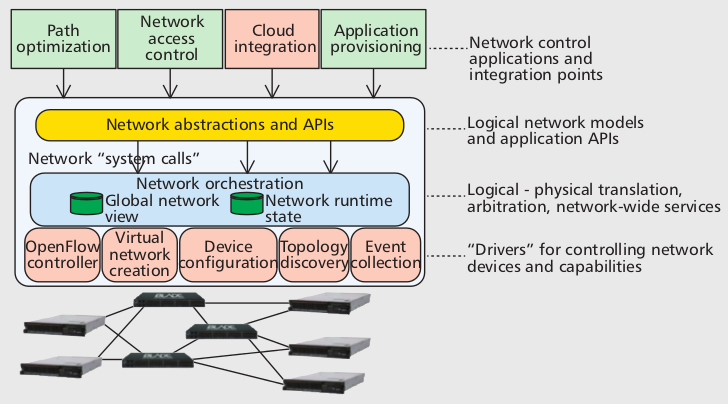
\includegraphics[width=0.8\textwidth]{figures/meridian_arch.png}
        \caption{Meridian SDN cloud networking platform architecture (Banikazemi et al.\cite{meridian})}
        \label{fig:meridian_arch}
\end{figure}

As shown in figure \ref{fig:meridian_arch}, the architecture is divided into three main layers: Network abstractions and API, where the network information can be accessed and manipulated (\textit{e.g.} access controlling policies, prioritizing traffic); Network Orchestration, translates the command provided by the API into physical network commands and orchestrates them for more complex operations. it also reveals the network topology and its variations; finally the ''drivers'' layer is an interface for underlying the network devices so several network devices and tools can be used.

Generally, this platform allows to create and manage different kind of logical network topologies and use their information for providing a greater control of the DC.
But as it works on top of a cloud Iaas platform (i.e., Openstack\cite{openstack}, IBM SmartCloud Provisioning\cite{scp}), it is limited to their management strategies and is only useful if one already has this type of infrastructure. Not having a testing environment is also a downside since the normal operation can be compromised and also alter the testing results.

\subsection{ICanCloud, GreenCloud and GroudSim}
\hspace{0.6cm}

Other well--known open--source cloud simulators are ICancloud\cite{icancloud}, GreenCloud\cite{greencloud} and GroudSim\cite{groudsim}, but in none of them SDN features are available.

\newpage
\subsection{Mininet}
\hspace{0.6cm}
\begin{quotation}

''Mininet is a network emulator which creates a network of virtual hosts, switches, controllers, and links. Mininet hosts run standard Linux network software, and its switches support OpenFlow for highly flexible custom routing and Software-Defined Networking.''

\hfill Mininet \cite{mininet}
\end{quotation}

As a network emulator for SDN systems, mininet can generate OF compliant networks that connect to real controllers without the need of hardware resources. Such features derives from the use of Open vSwitch and enables the assessment of the operation of an OF controller before its deployment in a real environment.

It also provides tools for automatically generating topologies, however, as they can be basic, an API is available to reproduce any type of topology and experiments.
Mininet hosts behave just like real hosts, can run any program as long as it does not depend on non linux kernels, and can send packets through emulated interfaces.
But as they share the same host file system and PID space, a special attention is required when killing/running programs.

Despite its flexibility, Mininet lacks of a complete set of tools that easily allow to emulate the behaviour of a cloud DC, thus raising the following questions:
 
\begin{itemize}
\item How to easily generate and configure typical DC topologies?
\item How to simulate VMs allocation requests?
\item How to emulate the inter and in/out DC traffic?
\end{itemize}

\newpage
\section{Openflow Controllers}
\hspace{0.6cm}


% Uncomment to include file.pdf
%\begin{figure}%[H]
%\begin{center}\includegraphics[scale=0.8]{file}\end{center}
%\caption{Legend \label{fig:LABEL}}
%\end{figure}


\chapter{The Framework \label{cha:framework} }
\hspace{0.6cm}

Provide the user with a full package for the development and test of DC SDN Controller was one of the main purposes of the framework.
Aiming for such goal, but without discarding the deployment in a real DC, a single software platform was designed and developed.
Because the requirements change according to the controller being in the development or the deployment phase, so does the platform by creating and environment that best suits each of them.

\section{Requirements}

\paragraph{Development \& Testing Phase}
\hspace{0.6cm}

-easy and fast to develop the desired logic 
  -easy access to information (switch and servers information, statistics)
  -easy management(installation/deletion) of OF Rules
  -automatic topology detection (switches and servers) on the controller
  -Easy communication with hypervisor

Testing environment
-VM Requests generator: generate automatic VM requests
-DC Topology generator: Tree and Fat tree topologies with variable breath
-Traffic generator: correctly "imitate" DC traffic from/to VM as they get allocated

\paragraph{Deployment Phase}
\hspace{0.6cm}

Ditch the whole testing environment
-place for people to make requests manually
-easy configuration

Explain the different requirements in a development \& test versus deployment phase.
 
This environment can be seen as two main components: the DC oriented controller and the DC Topology.

The first one, a full featured python controller for OF switches called POX was used as groundwork. It has ready-to-use modules that are helpful when it comes to making a controller, as they provide some abstraction.
However, POX API is too low level for a user that aims to implement a new DC controller, which prevents the rapid development of the logic thought by the user.
To fill this gap, the controller available in the framework includes all the abstraction levels needed for quickly building a DC oriented controller while still being fully dynamic.

As for the second component, since performing tests and debug in a real topology can be challenging operation

\section{Chosen technologies}
\hspace{0.6cm}

-Controller: POX
  -derives from the first OF controller made by the same people who created OF, which in some way should follow the same guidelines
  -Python as a programming language (higher level)
  -Object and Event oriented programming, more interactivity

-DC Emulator: Mininet
  -Chosen by OF as platform for testing OF controllers
  -Provides and API for development of custom made topologies and experiments (in python)
  -Although no traffic generator is included, hosts can run any program (with few restrictions)

-Virtualization platform: XCP 1.6 (Xen Cloud Platform)
  -Free and Opensource solution
  -Thought for the cloud
  -Xen python API

-Possibility to write all the code in one programming language helps keeping the platform consistent.
\newpage

\section{Framework architecture}
\hspace{0.6cm}

\begin{figure}[htbp]
        \centering
        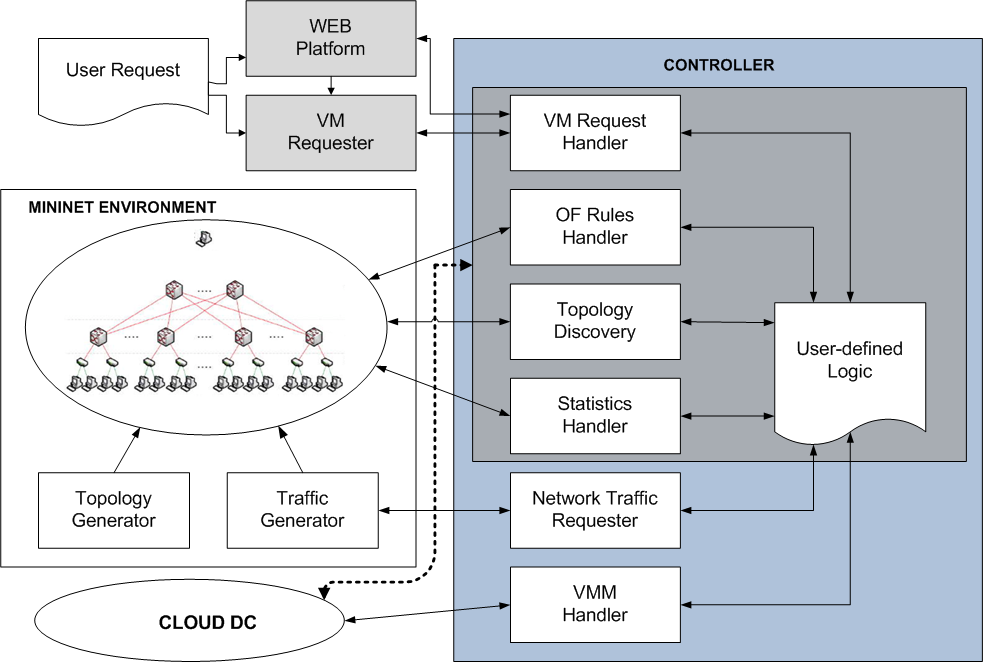
\includegraphics[width=0.8\textwidth]{figures/emulator_new.png}
        \caption{Framework Architecture}
        \label{fig:framework}
\end{figure}

The framework architecture, shown in figure \ref{fig:framework}, gives an overview of the its modules and their interaction.
The framework is divided into two main parts: the mininet environment - an extended version of mininet; and the controller - a modified, improved version of POX;

The mininet environment is made to be only used when testing the controller.
It is composed by the mininet platform with two extra modules that explore its API.
One of them is the {\it Topology Generator}, which allows to easily create a fat tree or tree DC topologies.
The other one is the {\it Traffic Generator} that allows to correctly simulate the allocation of VM into each server by generating traffic from that server to the exterior of the DC. It also allows to simulate inter VM communication.

As for the controller, it automatically manages the modules in order to only use the ones that are needed for each phase (testing or deployment).
In the figure \ref{fig:framework}, in the controller part, it can be seen a darker area which corresponds to the modules that are used in both phases. These modules are:
\begin{itemize}
  \item VM Request Handler -- Connects with the Web platform and/or the VM requester, and processes the VM requests.
  \item OF Rules Handler -- Manages and keeps track of the installation/removal of the OF rules from the switches.
  \item Topology Discover -- Manages all the information regarding the switches, links, servers and its detection.
  \item Statistics Handler -- Collects statistics about the switches and links, can be periodical or manual.
  \item User-defined Logic -- Space for the administrator/network engineer to develop the desired DC management logic
\end{itemize}

Regarding the other modules: the {\it Network Traffic Requester} which is only used when performing tests to tell the mininet environment how much, when, from where and where to the traffic should be generated; and the {\it VMM Handler} which in only active when the controller is in a real environment, and its purpose is to communicate with the hypervisor to do all the operation regarding the VMs (allocate, deallocate, upgrade, etc).

All the modules are independent from each other and they can be changed, removed or added in order to fulfill all the user requirements.


-Talk about the VM request how they can be made

\section{Framework modules: Mininet Environment}

\subsection{Topology Generator}

\subsection{Traffic Generator}

Describe each module, it's functionalities, limitations, how it can be used/improved (improved if the user wants to add new features)

\begin{itemize}
	\item Talk generally about the traffic generator
	\item Talk about the one's we tried (pros and cons)
\end{itemize}

\newpage


\section{Framework modules: Controller}

Describe each module, it's functionalities, limitations, how it can be used/improved (improved if the user wants to add new features)

\subsection{Topology Discovery}

\subsection{OF Rules Handler}

\subsection{Statistics Handler}

\subsection{VM Request Handler}

\subsection{VMM - Virtual Machines Manager}

\subsection{Network Traffic Requester}

\subsection{POX Modules}

\subsection{User Defined Logic}

\newpage


\section{Framework modules: Web Platform}

Describe each module, it's functionalities, limitations, how it can be used/improved (improved if the user wants to add new features)

\newpage


\section{Framework modules: VM Requester}

Describe each module, it's functionalities, limitations, how it can be used/improved (improved if the user wants to add new features)

\newpage


\section{Using the framework}

\subsection{Emulator}

Describe how to use the framework (emulation part) and how to access the API..

\subsection{Real Environment}

-Figura com o esquema da configuração
Describe what changes in the real environment (the modules that are disabled and the ones that need to be enabled)
\subsubsection{Real environment tests}
\begin{itemize}
  \item Talk about the environment which was setup
  \begin{itemize}
    \item Chosen hypervisor
    \item Talk about Xen api and the alternative solution (ssh each server and run a script to clone the vm)
    \item OpenVswitches VS NetFPGA problems
    \item 
  \end{itemize}
\end{itemize}

\section{Framework extensions \label{Sec:fraext} }

\subsection{Enabling QoS}
\subsubsection{State of art: QoS in SDN}
\subsubsection{QoS in the framework}
\newpage

\subsection{Enabling Virtual Machine migration}
\subsubsection{State of art: Virtual Machine migration}
\subsubsection{Virtual Machine migration in the framework}
\subsubsection{Usecase}

\chapter{Validation and tests \label{cha:valtes} }

Usually test and validation of the proposed solution ...

\section{Framework Validation}

\begin{itemize}
	\item Show how Bf goes against WF with server driven algorithm (show server occupation)
	\item Show how Bf goes against WF with network driven algorithm (show network occupation) (although the behaviour is similar is allow to say that net algorithm may use switch statistics)
\end{itemize}
\newpage


\section{Performance Evaluation}
\label{sec:perf}
\hspace{0.6cm}

TODO: CHANGE THIS FOR NOT BEING IN THE SECOND PERSON OF THE PLURAL
TODO: PUT IMAGES IN THE RIGHT PLACE (ALONG WITH THE TEXT)

We evaluated the actual performance of the proposed framework through a variety of experiments using a PC equipped with an Intel i5 3GHz and 8GB of DD3 RAM (\textit{i.e.}, from now on we will call it Host-PC).
The first tests have been carried out to inspect the impact of the amount of generated traffic, the DC topology size and the number of outside hosts on the host link ratio.
Firstly, we generate a static topology (\textit{i.e}, $2$ outside hosts, $2$ core switches, $4$ aggregation switches, $8$ edge switches, $8$ hosts), then we started measuring the host link ratio increasing the generated traffic per host.

\begin{figure}[htbp]
        \centering
        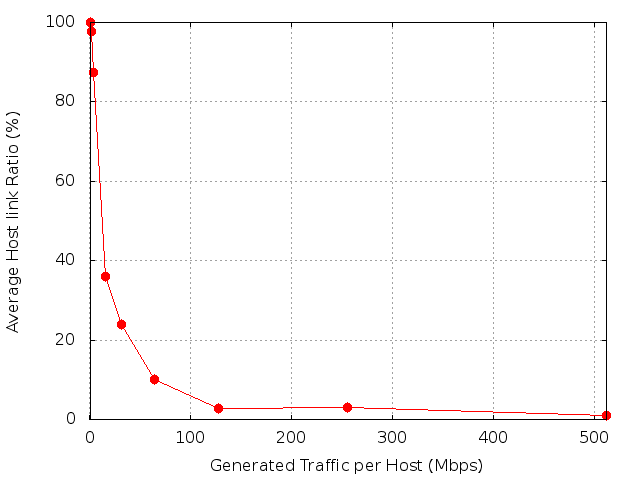
\includegraphics[width=0.6\textwidth]{figures/bw_utilization.png}
        \caption{Average Host link Ratio vs per Host Generated Traffic}
        \label{fig:bw}
\end{figure}

As shown in figure \ref{fig:bw} we were able to generate up to few Mbps of traffic per host.
Then the host link ratio decreases as the generated traffic grows.
We point out that such limitation does not affect any kind of DC performance tests made with our framework,
because we can scale the link speed as much as we want during the DC initialization phase, reaching every time 100\% of host link ratio.

\begin{figure}[htbp]
        \centering
        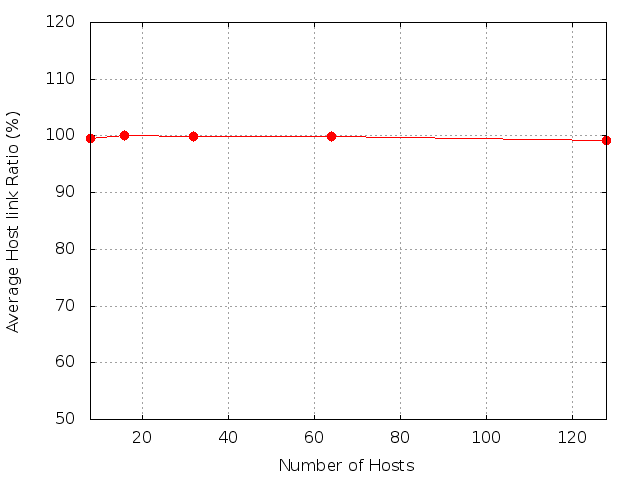
\includegraphics[width=0.6\textwidth]{figures/topo.png}
        \caption{Average Host Link Ratio vs number of Hosts}
        \label{fig:topo}
\end{figure}

In order to test the impact of the DC topology size on the
host link ratio we kept the amount of the generated aggregated traffic 
constant while exponentially increasing the number of switches and hosts.
We started from the previous test topology.

On DC initialization phase, we set the link speed in order to fully saturate the host links.

\begin{figure}[htbp]
        \centering
        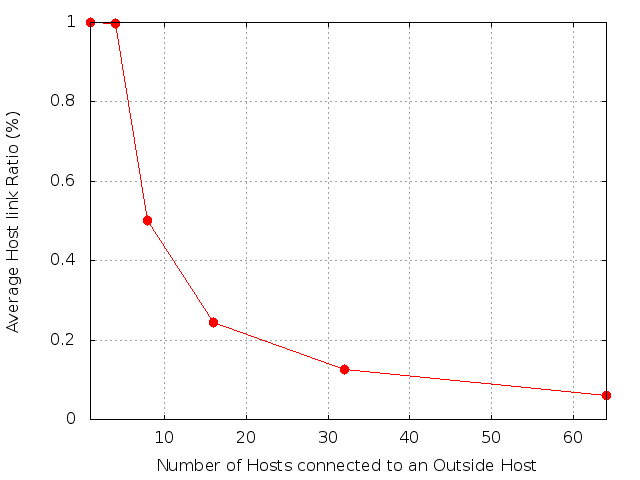
\includegraphics[width=0.6\textwidth]{figures/out_hosts_ratio.png}
        \caption{Average Host Link Ratio vs number of Hosts per Outside Host}
        \label{fig:hosts}
\end{figure}
\begin{figure}[htbp]
        \centering
        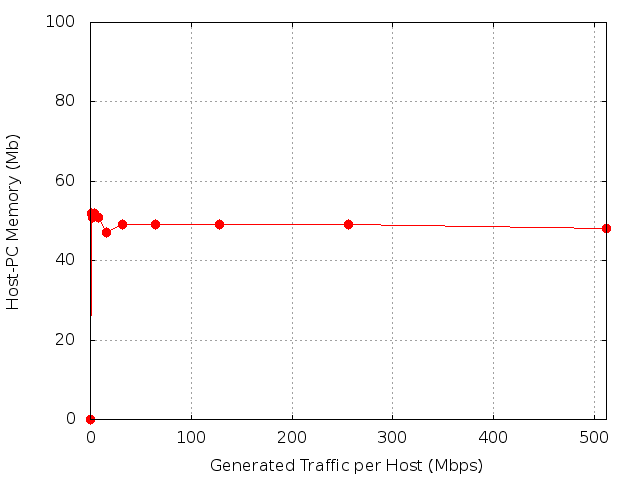
\includegraphics[width=0.6\textwidth]{figures/mem1_utilization.png}
        \caption{Host-PC Memory Utilization vs per Host Traffic Generated}
        \label{fig:mem1}
\end{figure}

The results in figure \ref{fig:topo} show that regardless of the hosts number, the host link ratio remains constant.
This means that as long as the total amount of generated traffic per host and the links speed can guarantee the link saturation, the system can scale indefinitely, being the only limits the Mininet itself, or the controller. 
Finally we investigated the relationship between the number of hosts connected to just one outside host and the average link ratio.
Figure \ref{fig:hosts} shows that a maximum of $8$ hosts can be managed by just one outside host (\textit{i.e.}, the host link speed is set in order to have a link saturation).

Such a result gives to the user an important constraint that should be used during the DC configuration phase.
We point out that this limitation is native of the Mininet environment and it is not due to our framework.
The second tests have been carried out to inspect the impact of both the amount of generated traffic and the DC topology size on the amount of memory the Host-PC needs.
Figure \ref{fig:mem1} shows that the memory utilization does not depend on the amount of generated traffic for each host.
On the other hand, as shown in figure \ref{fig:mem2}, as the topology size grows, the memory usage also grows in the same proportion, which allows to conclude that it scales linearly.

\begin{figure}[htbp]
        \centering
        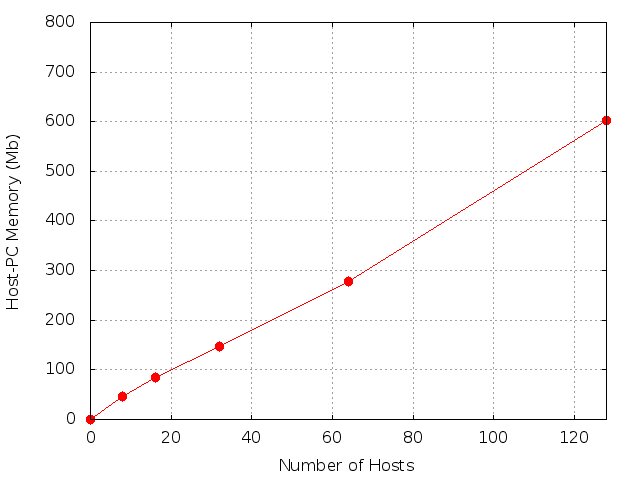
\includegraphics[width=0.6\textwidth]{figures/mem2_utilization.png}
        \caption{Host-PC Memory Utilization vs number of Hosts}
        \label{fig:mem2}
\end{figure}
\newpage

\chapter{Conclusions\label{cha:conclusions}}

This chapter provides ...

\section{Main contributions}

\section{Future work}

\appendix

\chapter{Name of the Appendix}

\cleardoublepage

\markright{\slshape Appendix}

\cleardoublepage
\bibliographystyle{unsrt}
\addcontentsline{toc}{chapter}{\bibname}

%% Add file.bib
\bibliography{sigproc}
\nocite{*}



\end{document}

%Layout do Vasco
% 0- Resumo/abstract
% 1- Conceitos Introdutórios
% WebRTC (APIs W3C)x, ICEx/STUNx/TURNx, RTP/DTLSx, Codecs, Protocolos DataChannel (UDP - SCTPx - DTLSx), Sinalização (draft JSEP, SIP sobre WebSockets, Jingle sobre WebSockets), WebSockets
% 2- Estado da Arte
% soluções existentes:
% Libs javascript incl as Libs do Muaz
% Sinalização: node.js, vertx
% Gateways para SIP
% 3- Requisitos e Casos de Uso
% 4- Experimentação e Seleção de Soluções Existentes
% Node.js vs Vertx
% Libs do Muaz vs ?
% 5- Arquitectura e Desenho
% Especificação das APIs Javascript e do Servidor (manual para programador)
% 6- Validação e Testes
% Aplicação 
% 7- Conclusões